\renewcommand{\vec}[1]{\mathbf{#1}} % my vector definition

\subsection{Self-adaptation in Evolution Strategies}
Mutation in evolution strategies is realized by adding normally
distributed random numbers to the components of the objective
vector. The choice of the variance of each normal distribution 
or in the general case the entries of the full
covariance matrix has been analyzed in depth and several 
proposals have been put forward. The most promising approaches
add the step-size parameters to the set-up of each individual and rely
on a ``second-order'' selection process for their choice. This is
termed self-adaptation of strategy parameters in ES. In the following, we
will give a short overview over the different methods, which are
implemented in the library.
%; the syntax of the different operators is
%summarized in Section \ref{classReference:sec:EALib}.

Whenever it is beneficial for the search process to move along the
e.\,g.\ $x_1$ coordinate in a specific proportion to the distance along the 
$x_2$ coordinate, we speak of the need for correlated mutations. In the
standard form correlated mutations are not accounted for, however all
asymmetrical problems (e.\,g. a rotated ellipsoid as a fitness
landscape) are likely to benefit from them. Therefore,
several schemes exist, which incorporate correlations between the 
variations. The most intuitive way is to rotate the matrix of
variances, as first proposed by Schwefel and described in
\cite{Baeck:96}. All other methods from the ``derandomized'' approach to 
self-adaptation in ES include correlated mutations in one way or the
other. The simplest method to adapt the complete correlation matrix is
difficult, since it cannot be guaranteed that the resulting system
will remain orthogonal and allow mutations in any direction 
(for this reason the number of vectors in the generating set 
approach in Section \ref{ss:GenSet} have to be consistently 
larger than $n$ (dimension of the search space).

Besides including correlated mutations along the axes, there is 
another approach to improve evolution strategies.
The ``derandomized'' adaptation mainly put forward by Ostermeier
\cite{Ostermeier:92,Ostermeier:94} aims at a more direct
adaptation of the strategy parameters. They argue that in the 
standard evolution strategy the adaptation has to overcome
the stochastic fluctuations which are introduced by the fact that even
distributions with small variances can produce large values and vice
versa. This source of ``noise'' in the adaptation process is
circumvented by using the actual step-length, that is the realization
of the random number $z$ for the adaptation. In addition, to the
derandomization the idea of an ``evolution path'' is inherent in all
of these approaches. The principle is very similar to a momentum term
in standard gradient descent approaches. The adaptation does not just 
rely on the step which is chosen in the current generation but also 
on selected steps in previous generation.

The following short overview introduces the
different strategies. More detailed information can be found in 
\cite{Baeck:96,Rechenberg:94,Schwefel:95} for Sections 
\ref{ss:standard} and \ref{ss:rotate}, in 
\cite{Hansen:98,Hansen:95,Ostermeier:94} for Sections \ref{ss:GenSet}
and \ref{ss:IndDir}, and in \cite{Hansen:98,Hansen:96} for Section
\ref{ss:CMA}.

\subsubsection{Standard adaptation}
\label{ss:standard}
In the standard evolution strategy, the mutation of the objective
variables $\vec{x}$ is carried out by adding a $N(0,\sigma_i^2)$ 
distributed random number $z_i$ to each component of $x_i$. The
``step-sizes'' $\sigma_i$ are also subject to mutations
(log-normal distributed) both for each component separately
(parameterized by $\tau$) and overall (parameterized by $\tau'$).
Thus, the individual consists of both the objective and the step-size 
vector. 
\begin{eqnarray}
\sigma_i(t) & = & \sigma_i(t-1) \exp( \tau' \, z) \; \exp( \tau \,z_i)\\
\vec{x}(t) & = & \vec{x}(t-1) + \vec{\tilde z}\\
z_i, z & \sim & N(0,1)\\
\vec{\tilde z}& \sim & N(\vec{0}, \vec{{\tilde \sigma}}(t)^2).
\end{eqnarray}
This is the
standard evolution strategy according to \cite{Baeck:96,Schwefel:95}.
The version put forward by \cite{Rechenberg:94} is different,
particularly with respect to the changes of the ``step-size'':
\begin{eqnarray}
\sigma_i(t) & = & \sigma_i(t-1) \,\xi,\\
\vec{x}(t) & = & \vec{x}(t-1) + \vec{\sigma}\cdot \vec{z}\\
z_i & \sim & N(0,1/n)
\end{eqnarray}
$\xi$ has the value $1.5$ with probability $\xi_{prob}$ and 
the value $1/1.5$ with probability $(1-\xi_{prob})$. In the standard
method in \cite{Rechenberg:94}, $\xi_{prob} = 0.5$.
$n$ is the dimension of the objective vector. The 
variance $1/n$ guarantees that the length $||z||$ is one on average
for large $n$.

\subsubsection{Rotation matrix adaptation}
\label{ss:rotate}
Instead of adapting the complete correlation matrix $\vec{C}$ of the
$n$-dimensional normal distribution (eq. \ref{fullCorr}), 
it is sufficient to rotate the diagonal matrix 
$\vec{C'}=diag(\sigma_1,\ldots,\sigma_n)$ using $n(n-1)/2$ rotation angles.
\begin{equation}
\label{fullCorr}
p(\vec{z}) = \frac{1}{(2\pi)^{n/2} \det \vec{C}}
\exp\left(-\frac{1}{2}\vec{z}^T\,\vec{C}^{-1}\,\vec{z}\right).
\end{equation}
The rotations can be written as follows using the rotation matrices
$\vec{R}(\alpha_{ij})$:
\begin{eqnarray}
\vec{R}(\alpha_{ij}) & = & \left( \begin{array}{ccccc}
1 & 0 & \cdots & \cdots &  0 \\
0 & 1 & \cdots & \cdots &  0 \\
\cdots & \cos \alpha_{ij} & \cdots & - \sin \alpha_{ij} & \cdots\\
\cdots & \cdots & \cdots & \cdots &  \cdots \\
\cdots & \sin \alpha_{ij} & \cdots & \cos \alpha_{ij} & \cdots\\
\cdots & \cdots & \cdots & \cdots &  \cdots \\
0 & \cdots & \cdots & 0 & 1
\end{array}\right)\\
\vec{{\tilde \sigma}} & = & \left( \prod^{n-1}_{i=1}\prod_{j=i+1}^{n}
\vec{R}(\alpha_{ij}) \right) \cdot \vec{\sigma}
\end{eqnarray}
The trigonometric functions occur in $\vec{R}(\alpha_{ij})$ at the
positions $(row, column) =(i,i), (i,j), (j,i), (j,j).$
Mutation of the $n$ step sizes $\vec{\sigma}$ and the mutation angles
is carried out like in the standard algorithm
\begin{eqnarray}
\sigma_i(t) & = & \sigma_i(t-1) \exp( \tau' \, z) \; \exp( \tau \,z_i)\\
\alpha_{ij}(t) & = & \alpha_{ij}(t-1) + \beta \,z^{\alpha}_{ij}\\
\vec{x}(t) & = & \vec{x}(t-1) + \vec{\tilde z}\\
z_i, z, z^{\alpha}_{ij} & \sim & N(0,1)\\
\vec{\tilde z}& \sim & N(\vec{0}, \vec{{\tilde \sigma}}(t)).
\end{eqnarray}
The values of $\alpha_{ij}$ are confined to the interval $[-\pi,\pi]$
and a lower bound can be defined for the $\sigma_i$ (in the function
this is determined by the values of {\em toggle} and $\epsilon$).
The standard setting of the parameters is shown in Table 
\ref{RotateParams}, two
versions of the operator {\sffamily\bfseries\small mutateRotate}
exist, one which includes the standard values and one where all
variables have to be defined explicitly. The composition of
the chromosome is shown in Figure \ref{StdBelegung} (a).

\begin{table}
\centerline{
\begin{tabular}{c|c|l}
\hline
Parameter & Standard Value & Comment \\
\hline
$\tau'$ & $1/\sqrt{2n}$  & heuristic value \\
$\tau$ & $1/\sqrt{2\sqrt{n}}$ & heuristic value \\
$\beta$ & $0.0873$  & heuristic value \\
{\em toggle} & FALSE & enforce lower bound \\
$\epsilon$ &   & lower bound for $\sigma$ \\
\hline
\end{tabular}}
\hfill\\
\caption[T1]{\label{RotateParams}Parameters for the rotation angle
  adaptation and their standard values; $n$ is the dimension of the
  objective vector $\vec{x}$.} 
\end{table}
\begin{figure}
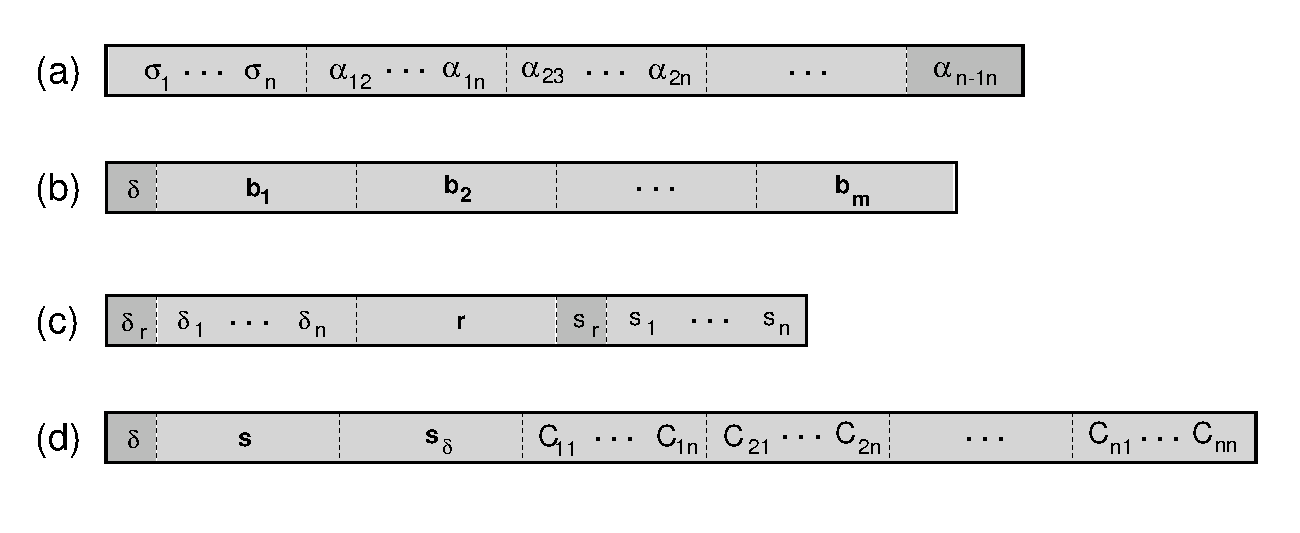
\includegraphics[width=0.7\columnwidth]{esStds.eps}
\caption{\label{StdBelegung}The position of the various mutation
  parameters for the different self-adaptation schemes in the chromosome
  \emph{stddev}. (a) Rotation matrix adaptation, 
  (b) generating set adaptation, (c) individual step sizes and 
  one direction adaptation, (d) covariance matrix adaptation.}
\end{figure}

\subsubsection{Generating set adaptation}
\label{ss:GenSet}
In the generating set adaptation (GSA) the random vector $\vec{y}$, which is
used to alter the objective vector $\vec{x}$, is a linear combination
of previous modifications $\vec{b}_i$, which have been selected,
multiplied by a normally distributed random value $z \sim
N(0,1)$. The previous vectors $\vec{b}_i$ make up the
generating set and serve as a kind of memory of successful earlier
steps taken on the fitness landscapes. Formally, we can write:
\begin{eqnarray}
\vec{y} & = & c_m \cdot \left( z_1 \vec{b}_1(t-1) + z_2 \vec{b}_2(t-1)
+ \ldots + z_m \vec{b}_m(t-1) \right);\quad z_i \sim N(0,1)\\
\label{GSeq2}
\vec{x(t)} & = & \vec{x(t-1)} + \delta(t-1)\, \xi \, \vec{y}
\end{eqnarray}
In equation (\ref{GSeq2}) $\delta$ and $\xi$ are overall step size 
parameters and $c_m$ is a normalization constant. The variation of the
mutation parameters is carried out as follows. 
\begin{eqnarray}
\delta(t)    & = & \delta(t-1) \, \xi^\beta \\
\label{bAdap1}
\vec{b}_i(t) & = & (1-c)\, \vec{b}_{1}(t-1) + c\cdot (c_u \xi) \, \vec{y}\\
\label{bAdap2}
\vec{b}_1(t) & = & \vec{b}_{1}(t-1)
\end{eqnarray}
The adaptation of the generating set in equation (\ref{bAdap1},\ref{bAdap2})
is intuitive. The oldest vector $\vec{b}_m$ is removed, the other
vectors are shifted one position and the new first vector is a linear
combination (the influence of the new vector is governed by the
parameter $c$) of the parent vector and the new variation vector
$\vec{y}$. $c_u$ again is used for normalization purpose. In Figure
\ref{GSAFigure} the adaptation of the generating set is shown.
The adaptation of the overall step size parameter $\delta$ is controlled by
the parameter $\beta$, $\xi$ has the value $1.5, 1/1.5$ with equal 
probability. There are two different versions of the function 
{\sffamily\bfseries\small mutateGSA}. The first receives the 
parameter vector \emph{stddev} (see Fig. \ref{StdBelegung})
as input. All the other constants are 
initialized with standard values as 
specified in \cite{Hansen:95}, see Table \ref{GenSetParams}. 
The second function receives explicit values for all parameters.
\begin{table}
\centerline{
\begin{tabular}{c|c|l}
\hline
Parameter & Standard Value & Comment \\
\hline
$c$ & $1/\sqrt{n}$  & heuristic value \\
$m$ & $\{n^2,\ldots,2n^2\}$ & heuristic value \\
$\beta$ & $1/\sqrt{n}$  & heuristic value \\
$c_m$ & $(1/\sqrt{m})(1+1/m)$ & normalization of $\vec{y}$ \\
$c_u$ & $\sqrt{(2-c)/c}$ & normalization of the variances \\
$\xi$ & $\{1.5,1/1.5\}$ & heuristic value\\
\hline
\end{tabular}}
\hfill\\
\caption[T1]{\label{GenSetParams}Parameters for the generating set
  adaptation and their standard values; $n$ is the dimension of the
  objective vector $\vec{x}$.} 
\end{table}
\begin{figure}
\centerline{
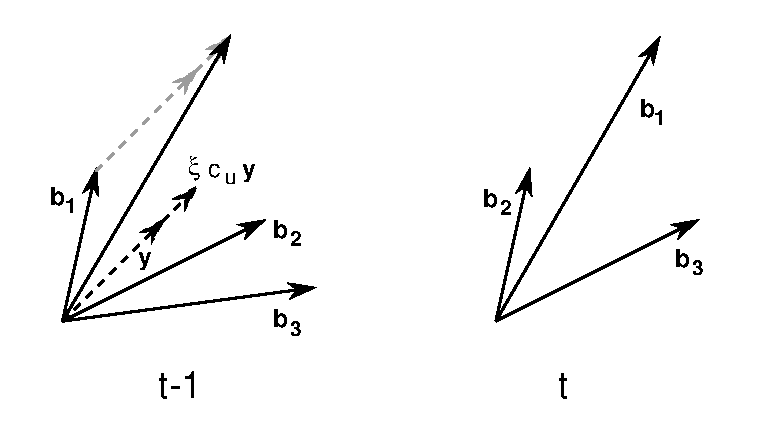
\includegraphics[width=0.6\columnwidth]{gsa.eps}}
\caption{\label{GSAFigure}Adaptation of the generating set from one
  generation to the next, as specified in equation
  (\ref{bAdap1},\ref{bAdap2}).}
\end{figure}


\subsubsection{Individual step sizes and one direction adaptation (IDA)}
\label{ss:IndDir}
With the introduction of a mutation in {\em one direction}, specified 
by $\vec{r}$, the problem of correlated mutations is circumvented. In
addition to the {\em one direction} mutation, $n$ (dimension of
the objective vector) individual step sizes for the different
coordinate axes are adapted. Therefore, the update of the objective vector
can be written as follows:
\begin{equation}
\label{IDAadap}
x_i(t) = x_i(t-1) + \delta_i(t-1)\,z_i + \delta_r(t-1)\,z\,r_i(t-1)
\end{equation}
The first term describes the individual step size mutation with
$z_i \sim N(0,1)$ and step sizes $\delta_i(t-1)$. In the second
term the direction $\vec{r}(t-1)$ is multiplied with the step
size $\delta_r(t-1)$ and the random variable $z \sim N(0,1)$.
The two different contributions to the overall mutation are shown 
in Figure \ref{IDAFig}. The adaptation of the step size parameters
and of the direction $\vec{r}$ relies on the ``derandomized'' approach and
on the averaging of the parameters over several generations. These
values are stored in $\vec{s}(t)$ and $s_r(t)$. The
accumulation time is determined by the parameters $c$ for the 
individual step sizes and $c_r$ for the direction:
\begin{eqnarray}
\vec{s}(t) & = & (1-c) \cdot \vec{s}(t-1) + c \cdot (c_u\,\vec{z})\\
\vec{r}(t) & = & \frac{1}{Norm} \,
                 (1-c_r) \cdot \delta_r(t)\, \vec{r}(t-1) + 
                 c_r \cdot (\vec{x}(t)-\vec{x}(t-1))\\
s_r(t)     & = & (1-c) \cdot s_r(t-1) + c \cdot (c_u\,z_r)
\end{eqnarray}
If $s_r(t)$ is smaller than zero, it is set to zero. $\vec{r}(t)$ is
normalized, thus $Norm=||\vec{r}(t)||$. Therefore $\vec{s}(t)$ and
$s_r(t)$ constitute memories for the random variations over the last
generations weighted by $c$. The direction vector $\vec{r}(t)$ also
includes such a generation memory. Lastly, the different step sizes
are adapted by log-normal distributions; the parameters 
$\hat{\chi}_n$ and $\hat{\chi}_1$ make sure that the expectation is
zero. For the adaptation of $\delta_r$ a lower bound is given by $\xi$
times the norm of the vector of the individual step sizes, in order not
to suppress the {\em one direction} mutation:
\begin{eqnarray}
\delta_i(t-1) & = &\delta_i(t)\;
\exp\left(\beta\left(||\vec{s}(t)||-\hat{\chi}_n\right)\right)\;
\exp\left({\tilde \beta}\left(|s_i(t)|-\hat{\chi}_1\right)\right)\\
\delta_r(t-1) & = &\delta_r(t)\;
\exp\left({\beta_r}\left(|s_r(t)|-\hat{\chi}_1\right)\right).
\end{eqnarray}
Again two different versions of {\sffamily\bfseries\small
  mutateIDA} are available in the EALib, one with predefined
values (see Table \ref{DirMutParams}) for the variables and one
  without. The composition of
the chromosome is shown in Figure \ref{StdBelegung} (c).

\begin{table}
\centerline{
\begin{tabular}{c|c|l}
\hline
Parameter & Standard Value & Comment \\
\hline
$c$ & $1/\sqrt{n}$  & heuristic value \\
$c_r$ & $3/n$  & heuristic value \\
$\beta$ & $2/n$  & heuristic value \\
${\tilde \beta}$ & $1/(4n)$  & heuristic value \\
$\beta_r$ & $1/(2\sqrt{n})$  & heuristic value \\
$\xi$ & $1/3$ & heuristic value\\
$\hat{\chi}_1$ & $\sqrt{2/\pi}$ & expectation of the $\chi_1$
distribution\\
$\hat{\chi}_n$ & $\sqrt{n} \left(1-\frac{1}{4n}+\frac{1}{21n^2}\right)$ &
expectation of the $\chi_n$ distribution (estimate)\\
\hline
\end{tabular}}
\hfill\\
\caption[T1]{\label{DirMutParams}Parameters for individual steps size
  and one direction adaptation and their standard values; 
  $n$ is the dimension of the objective vector $\vec{x}$.} 
\end{table}
\begin{figure}
\centerline{
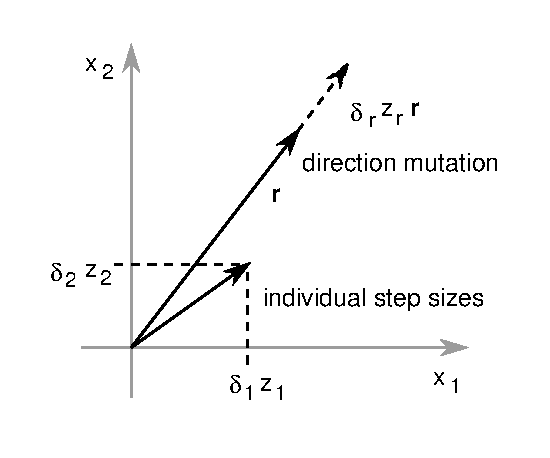
\includegraphics[width=0.5\columnwidth]{ida.eps}}
\caption{\label{IDAFig}The different contributions from the 
individual step size mutations and the direction mutation as specified
in equation (\ref{IDAadap}).}
\end{figure}

\subsubsection{Covariance matrix adaptation (CMA)}
\label{ss:CMA}
In the CMA algorithm the whole covariance matrix $\vec{C}$ as given in
eq. (\ref{fullCorr}) is adapted. The covariance matrix determines a
matrix $\vec{B}$, which is used to transform a random vector with
$N(0,1)$-distributed components into a vector which is
$N(\vec{0},\vec{C})$ distributed,
$\vec{C}=\vec{B}\vec{B}^T$. Therefore, the changes to the objective
variables can be written as 
\begin{equation}
\vec{x}(t) = \vec{x}(t-1) + \delta(t-1)\,\vec{B}(t-1)\,\vec{z},\quad
z_i \sim N(0,1)
\end{equation}
The adaptation of the covariance matrix occurs in two steps, again
averaged over the generations
\begin{eqnarray}
\label{vec_s}
\vec{s}(t) & = & (1-c)\, \vec{s}(t-1) + c_u\,\vec{B}(t-1)\,\vec{z}\\
\vec{C}(t) & = & (1-c_{cov})\, \vec{C}(t-1) + c_{cov} \, \vec{s}(t)\vec{s}^T(t)
\end{eqnarray} 
The parameter $c_u$ is introduced for normalization. It is interesting
to note that the CMA is closely connected to the GSA, see
\cite{Hansen:96}. The adaptation
over generations in eq. (\ref{vec_s}) can be seen as summing up
various mutation vectors (over the generations) to yield $\vec{s}$ from 
which in turn $\vec{C}$ is derived. In GSA this sum is realized in
each generation by all the vectors in the generating set. The next
step is to determine the matrix $\vec{B}$ from $\vec{C}$. Since 
$\vec{C}=\vec{B}\vec{B}^T$ is not sufficient to derive $\vec{B}$,
we choose as column vectors the eigenvectors of $\vec{C}$. The reason
is, that in the last step the overall step size $\delta$ has to be 
adapted. In order to perform the usual adaptation, we have to
know the expected length of the cumulative vector $\vec{s}_{\delta}$.
Therefore, the variation vector should be $N(\vec{0},\vec{I})$
distributed. We get
\begin{eqnarray}
\vec{s}_{\delta}(t) &=& (1-c)\,\vec{s}_{\delta}(t-1) + 
c_u\,\vec{B}_{\delta}(t-1)\,\vec{z}\\
\delta(t) & = & \delta(t-1)\cdot \exp\left(\beta\left(||\vec{s}_{\delta}(t)||-\hat{\chi}_n\right)\right)
\end{eqnarray}
$\vec{B}_\delta$ equals $\vec{B}$ with normalized columns in order for
$\vec{B}_{\delta}(t-1)\,\vec{z}$ to be $N(\vec{0},\vec{I})$
distributed. As in the other cases there are two different versions of
the function {\sffamily\bfseries\small mutateCMA}, with and
without standard values for the parameters shown in Table
\ref{CMAParams}. The composition of
the chromosome is shown in Figure \ref{StdBelegung} (d).

\begin{table}
\centerline{
\begin{tabular}{c|c|l}
\hline
Parameter & Standard Value & Comment \\
\hline
$c$ & $1/\sqrt{n}$  & heuristic value \\
$c_{cov}$ & $2/n^2$  & heuristic value \\
$\beta$ & $1/n$  & heuristic value \\
$c_u$ & $\sqrt{c (2-c)}$ & normalization of the variances \\
$\hat{\chi}_n$ & $\sqrt{n} \left(1-\frac{1}{4n}+\frac{1}{21n^2}\right)$ &
expectation of the $\chi_n$ distribution (estimate)\\
\hline
\end{tabular}}
\hfill\\
\caption[T1]{\label{CMAParams}Parameters for the covariance matrix
  adaptation and their standard values; 
  $n$ is the dimension of the objective vector $\vec{x}$.} 
\end{table}



%%% Local Variables: 
%%% mode: latex
%%% TeX-master: "EALib-standalone"
%%% End: 
